\section{Wstęp}


Naiwny klasyfikator Bayesa jest prostym klasyfikatorem probabilistycznym opartym na twierdzeniu Bayesa. Nazywany jest naiwnym ze względu na przyjęte założenie, które mówi, że poszczególne cechy są wzajemnie niezależne. Pomimo tak dużego uproszczenia, klasyfikator wypada niespodziewanie dobrze w wielu rzeczywistych problemach. Dużą zaletą tego klasyfikatora jest dobra skalowalność, metoda operuje jedynie na jawnych wzorach w przeciwieństwie do innych metod wykorzystujących podejście iteracyjne.

Jednym z zastosowań klasyfikatora jest diagnozowanie wad i dysfunkcji serca na podstawie sygnału EKG, a dokładniej występującego w nim zespołu QRS. Jest to zespół opisujący pobudzenie mięśni serca. Uproszczony przebieg EKG z zespołem QRS został umieszczony na rysunku \ref{fig_qrs}.

\begin{figure}[!htb]
  \begin{center}
    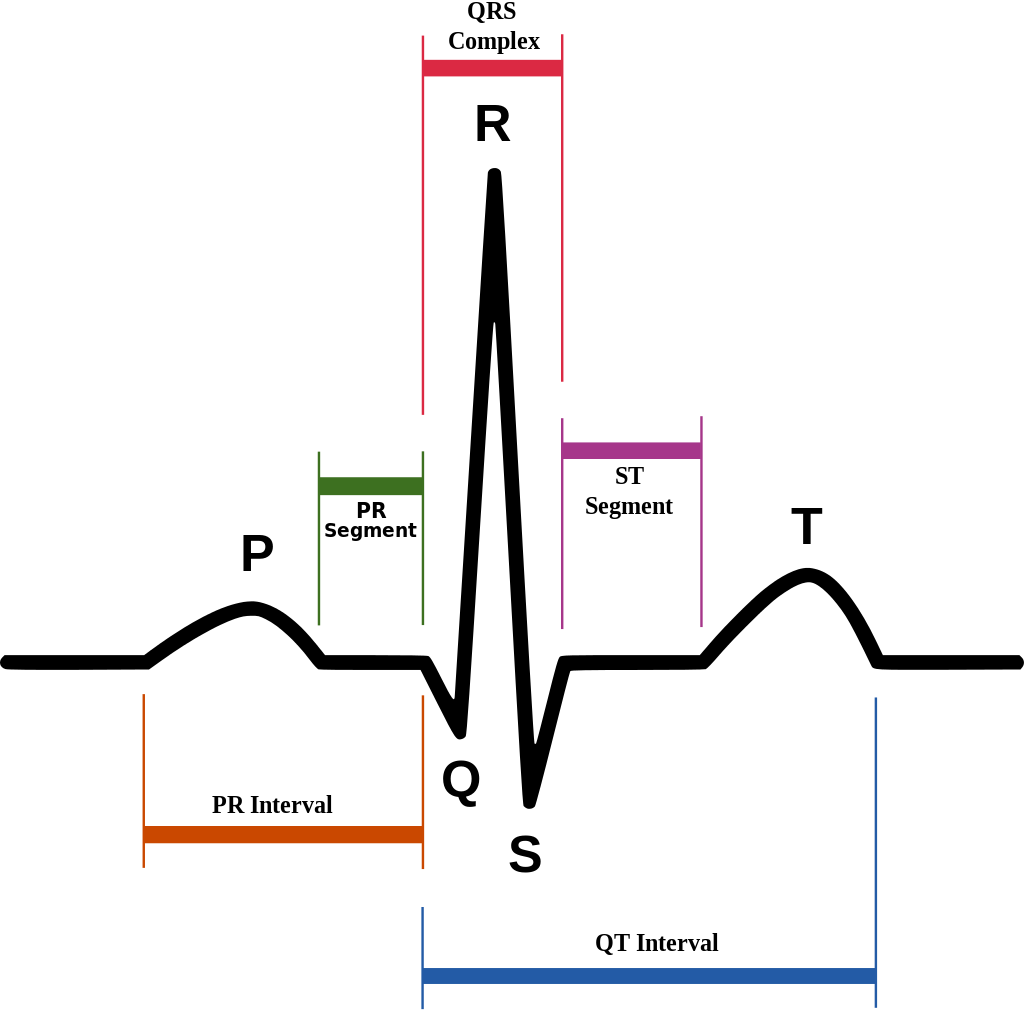
\includegraphics[scale = 0.25]
    {img/qrs.png}
  \end{center}
  \caption{Uproszczony zespół QRS - źródło \ref{}}
  \label{fig_qrs}
\end{figure}

W celu dokonania klasyfikacje konieczne jest zdefiniowanie wskaźników opisujących QRS. Na podstawie rysunku \ref{fig_qrs} możemy wyróżnić następujący cechy:

	\begin{itemize}
	\item{Wartość szczytowa załamka R i moment jej wystąpienie} 
	\item{Odstęp pomiędzy wcześniejszym a obecnie analizowanym załamkiem R}
	\item{Odstęp pomiędzy aktualnie analizowanym i kolejnym załamkiem R}
	\item{Początek/koniec oraz początkowa/końcowa wartość załamka P}
	\item{Wartość szczytowa załamka P i moment jej wystąpienia}
	\item{Początek/koniec i wartość początkowa/końcowa całego zespołu QRS}
	\item{Wartość szczytowa załamka T i moment jego wystąpienia}
	\item{Koniec i wartość końcowa załamka T}
	\end{itemize}